
%%% Local Variables:
%%% mode: LaTeX
%%% TeX-master: t
%%% End:




%\usepackage[sorting=none,backend=biber]{biblatex}

\begin{document}

%%% Local Variables: 
%%% coding: utf-8
%%% mode: latex
%%% TeX-engine: xetex
%%% End:

%%% Титульный лист
\begin{titlepage}
\begin{center}
Министерство образования Республики Беларусь\\[1.2em]
Учреждение образования\\[0.4em]
БЕЛОРУССКИЙ ГОСУДАРСТВЕННЫЙ УНИВЕРСИТЕТ ИНФОРМАТИКИ И РАДИОЭЛЕКТРОНИКИ\\[2.0em]
\end{center}

\vfill
\begin{center}
\textbf{ОТЧЕТ}\\
к лабораторной работе №3 на тему:\\
\textbf{ОПРЕДЕЛЕНИЕ НАДЕЖНОСТИ ТЕХНИЧЕСКОЙ СИСТЕМЫ}\\
\textbf{МЕТОДОМ ПРЯМОГО ПЕРЕБОРА ЕЁ РАБОТОСПОСОБНЫХ СОСТОЯНИЙ}\
\end{center}

\vfill
\begin{flushright}
    \begin{minipage}{9.3cm}
        Студент:  гр. 112601 Корякин~А.~Л.\\[0.1em]

        Отчет представлен на проверку: \underline{\hspace*{1.4cm}}.\underline{\hspace*{1.4cm}}.2024\\
        \underline{\hspace*{5.6cm}}
        
    \end{minipage}
  \end{flushright}
  
  \vfill
  \begin{center}
    {\normalsize Минск 2024}
    \end{center}

  \end{titlepage}


\section*{Цель лабораторной работы}

Определить показатели надёжности РЭУ моделированием на ПЭВМ
отказов элементов.

Ознакомиться с математическим описанием основных законов распределения
времени до отказа элементов.
Исседовать моделированием на ПЭВМ влияние параметров законов
распределения надёжности.
Определить моделированием на ПЭВМ показтели надёжности РЭУ
при одинаковых и различных законах распределния времени
до отказа элементов.

\section{таблица координат эксперементальных точек}
	

\begin{table}[H]
  \centering
  \begin{tabular}{| l | c | r |}
    \hline
  $ \lambda_{n} $ &  Лямбда	&  Среднее время   \\ \hline
  $ \lambda_{1} $ &  0,0001	&  10135,33        \\ \hline
  $ \lambda_{2} $ &  0,00025	&  3759,529        \\ \hline
  $ \lambda_{3} $ &  0,00075	&  1358,138        \\ \hline
  $ \lambda_{4} $ &  0,001	&  1009,236        \\ \hline
  $ \lambda_{5} $ &  0,005	&  189,5253        \\ \hline
  $ \lambda_{6} $ &  0,0075	&  141,3908        \\ \hline
  $ \lambda_{7} $ &  0,01	&  101,5989        \\ \hline
	
  \end{tabular}  
  \caption{Таблица с координатами эксперементальных точек
    по результатам моделировани}
\end{table}

\section{график по данным таблицы}


\graphicspath{ {img} }
\begin{figure}[H]
  \centering
  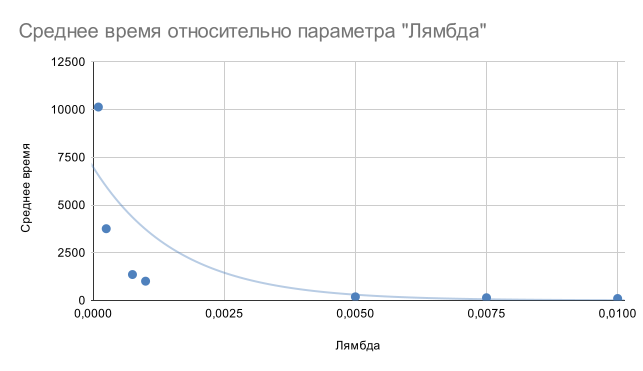
\includegraphics[scale=0.6]{avg-to-lambda.png}
  \caption{График зависимости $T_\textrm{ср} = f ( \lambda )$ построенный по данным таблицы}
\end{figure}


\section{результаты исследования надёжности}

Результаты исследования надёжности (вероятности безотказной рабо-
ты) двух элементов, имеющих нормальное распределение времени до отказа,
но с разными значениями параметров $t_{\textrm{ср}}$ и $\sigma_{t}$.
\begin{figure}[H]
  \centering
  \includegraphics[scale=0.15]{part2.png}
  \caption{Cкриншот программы с проведенным исследованием.}
\end{figure}

На приведенном скриншоте видно как при большем $t_{\textrm{ср}}$
меньше $P(t_{\textrm{з}})$.

\begin{figure}[H]
  \centering
  \includegraphics[scale=0.2]{t-avg-geom-half.png}
  \caption{График площадь под которым считается за вероятность отказов}
\end{figure}
Элемент взятый из партии с меньшим значением
показателя $t_{\textrm{ср}}$ имеет большую вероястность
безотказной работы для времени $t_{\textrm{з}}$ = 5000ч,
потому что при таком значении
оказывается меньшей площадь под графиком,
численно равная $P(t_{\textrm{з}})$.


\section{сравнительная оценка показателей безотказности для случая
  \newline экспоненциального распределения
  \newline времени до отказа}

\begin{figure}[H]
  \centering
  \includegraphics[scale=0.2]{part3.png}
  \caption{Cкриншот программы с проведенным исследованием.}
\end{figure}

Таким образом, получаются следуюшие значения

\begin{table}[H]
  \centering
  \begin{tabular}[c]{| l | c | r |}
    \hline
    $\lambda$  & $P(T_{\textrm{з}})$ & $T_{\gamma}$ \\ \hline
    $\lambda_{1}$ = 0,000015 & 0,9 & 1003,7 \\ \hline
    $\lambda_{2}$ = 0,000035 & 0,9 & 1003,7 \\ \hline
    $\lambda_{3}$ = 0,000045 & 0,9 & 1003,7 \\ \hline
    \hline
  \end{tabular}
  \caption{Значения полученные моделированием}
\end{table}

$T_{\textrm{ср}}$ вычисляется по формуле $T_{\textrm{ср}} = \frac{1}{\lambda}$.\\

$P(T_{\textrm{з}})$ вычисляется по формуле
$P(T_{\textrm{з}}) = e ^{- \lambda t_{\textrm{з}}}$.\\

$T_{\gamma}$ вычичсляется
по формуле $T_{\gamma} = -T_{\textrm{ср}}ln (\frac{\gamma}{1000})$

\begin{table}[H]
  \centering
  \begin{tabular}[c]{| l | c | c | r |}
    \hline
 $\lambda$ & $T_{\textrm{ср}}$ & $P(T_{\textrm{з}})$ & $T_{\gamma}$ \\ \hline
$\lambda_{1}$ = 0,000015 & 66666.667 & 1,077884  & 7023 \\ \hline
$\lambda_{2}$ = 0,000035 & 28571.429 & 1,192146  & 3010 \\ \hline
$\lambda_{3}$ = 0,000045 & 22222.222 & 1,252323 & 2341 \\ \hline
    \hline
  \end{tabular}
  \caption{Значения полученные аналитически}
\end{table}

\section{сравнительная оценка показателей безотказности  для случая
  \newline разных законов распределения
  \newline времени до отказа}
%Таблица 1.4

\begin{figure}[H]
  \centering
  \includegraphics[scale=0.2]{part4.png}
  \caption{Cкриншот программы с проведенным исследованием.}
\end{figure}

\section{Вывод}


На практике для решения практических задач прибегают к методам моделирования из-за следующих причин: нет необходимости прибегать к экспериментам, экономит временяю,
помогает создать и разобрать ситуации для обучения будущих специалистов.

При получении случайных реализаций времени до отказа изделия во внимание принимают:
условия эксплуатации, качество сборки, метод крепления и сборки, качество компонентов и режим работы.

Экспоненциальный закон используется для описания времени до отказа большинства отечественных и зарубежных элементов.
Распределение Вейбола используется для полупроводниковых приборов и интегральных микросхем.
Нормальный закон распределения использует для элементов, работа которых сопровождается заметными процессами старения и износа.
Расхождение показателей, может быть, из-за: неучтенных факторов, использовании разных моделей расчетов, округления чисел при расчете.


\end{document}
